\newpage
\setcounter{secnumdepth}{3}
\section{Programming: RNN and Transformer in PyTorch [45 pts]}

In this programming task, you will implement an RNN and an encoder-only Transformer in PyTorch. The task we will be working on is a binary classification task on text data; your neural networks will predict whether each text sequence exhibits positive sentiment or negative sentiment. This programming section is worth 45 points: 13 points for the RNN autograder, 13 points for the Transformer autograder, 9 points for Questions 5.4.1–5.4.2, and 10 points total for Question 5.4.3, including its report and autograder submission. 

\textbf{Important Note on PyTorch:} In this programming task you are REQUIRED to use the automatic differentiation in PyTorch. You are allowed to use most of the built-in neural network modules in PyTorch (such as nn.Linear, nn.ReLU, nn.Softmax, etc.)\ unless otherwise specified.

\textbf{
PyTorch modules that are NOT allowed in this task: 
\begin{enumerate}
    \item All recurrent layers: nn.RNNBase, nn.RNN, nn.RNNCell, nn.LSTM, nn.LSTMCell, nn.GRU, nn.GRUCell
    \item All attention and Transformer layers: nn.MultiheadAttention, nn.Transformer, \\
    nn.TransformerEncoder, nn.TransformerEncoderLayer
\end{enumerate}
}

\subsection{The Yelp Dataset}
The dataset used in this assignment is the Yelp dataset, the same dataset used in the programming section of Homework 2. This dataset uses polarized labels, where reviews with 1 and 2 stars are labeled negative (``0" label) and reviews with 4 and 5 stars are labeled positive (``1" label). This specific dataset can be found  \href{https://huggingface.co/datasets/fancyzhx/yelp_polarity}{at this link} (though you don't need to download it from there, see our dataloader below) and is a subset of the full Yelp reviews dataset. This polarized version contains 598K text reviews (560k for training, 38k for testing) of various types of establishments, and we have further subsampled it to 15\% of the original size, such that the training set and testing set have 84k and 5.7k samples respectively.

The Yelp dataset will be loaded from the Hugging Face file system via Pandas. Each entry of the dataset contains 2 columns, the review text and its polarized label.

\subsubsection{Provided Dataloader}
For efficiency, we will only take the first $L=50$ words in each review for training and testing. We provide a dataset class and function to initialize the dataset and the dataloader for you in \texttt{reference\_data.py}. \textbf{Please carefully read and make sure you understand all the code in this file.}

The \texttt{reference\_data.py} class preprocesses the text reviews by translating each word into an index representing that word. The word-to-index mapping is stored in the \texttt{self.word\_dict} variable. Note that we include an additional padding token ``PAD'' that has index 0. We append the padding token to reviews that have lengths less than $L$, so that all reviews have the same length and can be batched together.

The dataloader will return a tuple containing the text tensor and the label tensor. If $B$ is the batch size, then the text tensor has shape $(B, L)$, where each element represents the dictionary index of the word at that specific position. The label is a one-dimensional tensor with length $B$.

\subsection{Implementing an RNN}

\subsubsection{Word Embedding} To convert the word indices into a word embedding, create an embedding layer using \texttt{torch.nn.Embedding}. The embedding layer takes in batched, word-index tensors with shape $(B, L)$ and outputs an embedding $\Xv$ with shape $(B, L, D_e)$, where the hyperparameter $D_e$ is the embedding dimension. The embedding layer maintains the embedding table tensor of shape $(N, D_e)$ that will be optimized during training. $N$ is the number of words in the dictionary. The $k$-th row in the embedding table will be the output vector corresponding to the input word at index $k$. Note that for the padding token ``PAD'' with index 0, we want to enforce its embedding to be a zero vector. % See PyTorch documentation on how to enforce this.

\subsubsection{LayerNorm} 

We covered layer normalization in class. It computes the mean and variance of a tensor across the feature dimension (as opposed to the batch dimension in batch normalization) and normalizes the tensor with respect to the computed mean and variance. It then learns a new mean and variance for the output and scales the normalized tensor according to those learned parameters. You should use \texttt{nn.LayerNorm} to perform layer normalization in your networks. Please see the equation below in Section~\ref{sec:RNN} to see where LayerNorm should be applied in the RNN layers.

\subsubsection{RNN} 
\label{sec:RNN}

\begin{center}
\begin{tikzcd}[cells={nodes={draw=gray}}]
	& {\hat{y}_1} & {\hat{y}_2} & {\hat{y}_3} \\
	{h_0} & {h_1} & {h_2} & {h_3} \\
	& {x_1} & {x_2} & {x_3}
	\arrow[from=2-1, to=2-2]
	\arrow[from=2-2, to=2-3]
	\arrow[from=2-3, to=2-4]
	\arrow[from=3-4, to=2-4]
	\arrow[from=3-3, to=2-3]
	\arrow[from=3-2, to=2-2]
	\arrow[from=2-2, to=1-2]
	\arrow[from=2-3, to=1-3]
	\arrow[from=2-4, to=1-4]
\end{tikzcd}
\end{center}

Given a working dataloader and embedding layer, we will now implement a simple RNN with one hidden layer. (Note: this is \emph{not} the same as the RNN you worked with in the written section above; e.g., that one had no LayerNorm.) The structure of the network is shown in the above diagram. $\xv_i, \hv_i, \hat{\yv}_i$ represents the input word embedding, hidden state, and output at the $i^{\textrm{th}}$ recurrent step respectively. Your network should contain three linear layers: input-to-hidden, hidden-to-hidden, and hidden-to-output layer, with weights represented by $\Wv_{xh}, \Wv_{hh}$, and $\Wv_{hy}$ respectively. You should initialize $\hv_0$ as a zero vector. Given the previous hidden state $\hv_{i-1}$ and the $i$-th word embedding $\xv_i$, you can compute $\hv_i$ and $\hat{\yv}_i$ as
\[
\hv_i = \tanh(\textrm{LayerNorm}(\Wv_{hh} \hv_{i-1} + \Wv_{xh} \xv_i)), 
\]
\[
\hat{\yv}_i = \textrm{softmax}(\Wv_{hy} \hv_i).
\]

\subsubsection{Loss and Prediction} Our RNN computes an output at every recurrent step. \textbf{Important:} You need to compute the loss for all of the outputs and sum over the recurrent steps to compute your total loss for each iteration. Use \texttt{nn.CrossEntropyLoss} as the loss criterion. During training, the same label should be used to calculate the loss for each output in the entire sequence, which is then summed over. However, for prediction, we only take the output at the very last recurrent step $\hat{\yv}_L$, and predict the label by taking the argmax of the last output.

\subsubsection{Train and Test your RNN} 

After finishing your RNN implementation, initialize your model, optimizer, and loss function. For this assignment, please use the Adam optimizer. 

You are also asked to write training and testing loops over the training dataloader. For each batch of inputs, run the forward and backward passes, then update the model using the optimizer. Train your model using the hyperparameters specified in the starter code. For testing your model, loop over the test dataloader and run a forward pass with \texttt{torch.no\_grad()}. 

Please log the average loss and prediction accuracy at each epoch in both your training and testing loop, as you will be asked to report and plot these values for your written responses in this section.

\subsection{Implementing a Transformer}

\subsubsection{Transformer Embedding} 

For the Transformer, we will use the same method as described above to convert word indices into embeddings. However, on top of that, we also need to incorporate positional encodings that provide the model information on the relative location of each token in the sequence. We add the positional encoding to the word embedding as the input to the model. The class \texttt{TransformerEmbedding} does this and is provided for you in the starter code. This positional encoding  follows the implementation described in ``Attention Is All You Need" (Vaswani et. al., 2017).

\subsubsection{Multi-head Attention Layer}

Implement the \texttt{AttentionLayer} class and then the \texttt{MultiHeadAttention} class. For single-head attention, given input $\Xv$ with shape $(B, L, D_e)$.
\[
\Qv = \Wv_Q \Xv, \ \Kv = \Wv_K \Xv, \ \Vv = \Wv_V \Xv
\]
where adjacent tensors denotes a batched matrix multiplication (or equivalently, tensor contraction) operation, $\Qv$ has shape $(B, L, D_Q)$ and $D_Q$ is the dimension of $\Qv$; $\Kv$ and $\Vv$ behave similarly. Note that the dimensions of $\Qv$ and $\Kv$ must be the same. 

Now we can compute the attention score and the final output of the attention layer as
\[
\textbf{ \textit{score} } = \textrm{softmax}\left(\frac{\Qv \Kv^{\intercal}}{\sqrt{D_Q}}\right), \ \zv = \textbf{ \textit{score} } \ \Vv
\]
where $\textbf{ \textit{score} }$ has shape $(B, L, L)$, $\zv$ has shape $(B, L, D_V)$, and $D_V$ $D_Q$ are hyperparameters (additionally, note that the transpose does not operate over the batch dimension). 

Multi-head attention with $N$ heads should contain $N$ attention layers. It computes outputs for each attention head and concatenates the outputs $\zv_1, \zv_2, \dots, \zv_N$. The concatenated output has shape $(B, L, N \times D_V)$. 

Lastly, we pass this output through a linear layer to reduce the dimension from $N \times D_V$ to $D_{model}$, giving a final output of shape $(B, L, D_{model})$.

\subsubsection{Transformer}

\begin{center}
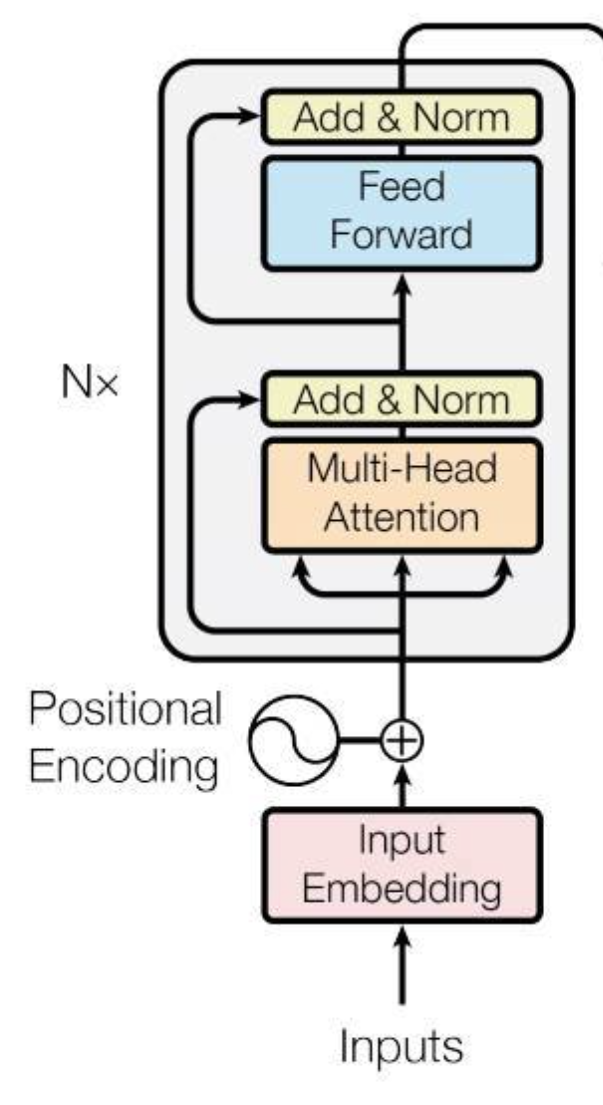
\includegraphics[height=6cm]{figures/transformer_encoder.png}
\end{center}

The structure of a Transformer encoder layer is shown in the above figure. (We will use an encoder-only architecture.)

Given input $\Xv$, it computes the intermediate tensor $\zv$ and output $\hat{\yv}$ as
\[
\zv = \textrm{LayerNorm}(\Xv + \textrm{MultAttn}(\Xv)), \ \hat{\yv} = \textrm{LayerNorm}(\zv + FF(\zv))
\]
where MultAttn represents multi-head attention and $FF$ represents a feed-forward network. The $FF$ network should consist of two linear layers and one ReLU activation after the first linear layer. Note the residual connections (add back in $\Xv$ when computing $\zv$, add back in $\zv$ when computing $\hat{\yv}$). Also note that we perform layer normalization \emph{after} each residual connection. In your implementations, $\zv$ and $\hat{\yv}$ should have the same shape as input $\Xv$. Implement the \texttt{FeedForward}, \texttt{Residual}, and the \texttt{EncoderLayer} classes. The Transformer contains multiple \texttt{EncoderLayer} modules and passes the input embedding through all the layers sequentially. The starter code gives the hyperparameters you should use (e.g., width of the FF network and number of Transformer layers).

\subsubsection{Loss and Prediction}

For loss and prediction, we will use the output of the \emph{first} word token ``SOS'', a dummy ``start of sentence" token we add to each text review. We pass this output through one more linear layer to reduce the dimension to 2, the number of classes in our task. Please use \texttt{nn.CrossEntropyLoss} for the loss and \texttt{argmax} to translate the model output to labels.

\subsubsection{Train and Test your Transformer} 

We encourage you to reuse the same code you wrote for training and testing your RNNs to train and test your Transformers. 



\newpage

\subsection{Empirical Questions}

\begin{enumerate}
    \item \textbf{[4 pts]} Train both the RNN and the Transformer encoder for 10 epochs using the hyperparameters specified in the starter code. Report the final accuracy of both models on both the test dataset and the training dataset. Report values up to the 4th decimal place. 
    
    \begin{tcolorbox}[fit,height=1.5cm, width=8cm, blank, borderline={1pt}{-2pt}]
        RNN Training Accuracy: 

    \end{tcolorbox}
    \begin{tcolorbox}[fit,height=1.5cm, width=8cm, blank, borderline={1pt}{-2pt}]
        RNN Test Accuracy:
  
    \end{tcolorbox}
    \begin{tcolorbox}[fit,height=1.5cm, width=8cm, blank, borderline={1pt}{-2pt}]
        Transformer Training Accuracy: 

    \end{tcolorbox}
    \begin{tcolorbox}[fit,height=1.5cm, width=8cm, blank, borderline={1pt}{-2pt}]
        Transformer Test Accuracy: 

    \end{tcolorbox}
    
    \item \textbf{[5 pts]} Describe the relationship between the values you reported in the previous question: does one model significantly outperform the other? Provide an explanation for the relative performances of the two models using what you know of the task and how we preprocessed the dataset.
    \begin{tcolorbox}[fit,height=6cm, width=15cm, blank, borderline={1pt}{-2pt}]
        %%% Write your solution here %%%

    \end{tcolorbox}

    \clearpage

    \clearpage
    
    \item \textbf{[10 pts]} Now we want to give you a chance to experiment with Transformers by exploring ways to enhance performance. You will need to implement one of the non-trivial enhancements listed below and write a report on your findings. In other words, your report should \textbf{not} just be tuning hyperparameters. Your report should include: 

    \begin{enumerate}[label=(\alph*)]
        \item A plot that shows the train and test loss for your newly enhanced Transformer.
        \item Model size (number of parameters).
        \item A description of the improvement(s) you made. 
        \item The set of hyperparameters you used (if it differs from the ones given). E.g., you could consider changing embedding dimension (\verb|d_model|) or number of transformer layers (\verb|n_layers|).
        \item The time required to train the model.
        \item An analysis your results in terms of improvements you made and the hyperparameters you used.
    \end{enumerate}

    Please implement one of the following major changes to your encoder-only transformer and report the effect on performance:
    \begin{itemize}
    \item \textbf{SwiGLU}: Replace the standard feed-forward network with SwiGLU, a gated linear unit that combines a linear transformation with a sigmoid-activated gate. This can enhance the model's expressiveness and has been shown to improve performance in large language models.~\footnote{https://arxiv.org/abs/2002.05202}
    \item \textbf{Switch from Post to Pre Normalization}: Transition to pre-normalization, where layer normalization is applied before the attention and feed-forward computations, as used in models like Llama. This can improve training stability, especially for deeper architectures.~\footnote{On Layer Normalization in the Transformer Architecture
 (https://arxiv.org/abs/2002.04745)}
    \item \textbf{Relative Positional Encodings}: Integrate relative positional encodings into the attention mechanism to dynamically capture the relationships between tokens. Unlike fixed absolute encodings, relative encodings model the distance between tokens, enabling the model to generalize better.~\footnote{Self-Attention with Relative Position Representations (https://arxiv.org/abs/1803.02155)}
    \item \textbf{RoPE (Rotary Positional Embeddings)}: Implement RoPE, which encodes positional information using rotation matrices. Note, this can be challenging to implement from scratch. It is most useful for handling longer sequences and is used in advanced models.~\footnote{RoFormer: Enhanced Transformer with Rotary Position Embedding (https://arxiv.org/abs/2104.09864)}
    \item \textbf{Other Changes}: Consider additional modifications such as using different activation functions like GELU~\footnote{Gaussian Error Linear Units (https://arxiv.org/abs/1606.08415)} or using RMSNorm instead of LayerNorm for potentially more efficient normalization.~\footnote{Root Mean Square Layer Normalization
 (https://arxiv.org/abs/1910.07467)}
    \end{itemize}
    

    \textbf{Important Requirements}: 
     \begin{itemize}
        \item Your model size should \textbf{not} be more than 3M parameters. 
        \item You \textbf{must} include at least one of the listed non-trivial enhancements to your Transformer. Simply tuning hyperparameters will not result in full points.
    \end{itemize}

    In addition to your report below, please submit your ‘‘predicted\_labels.pkl" file to the autograder in the separate Gradescope assignment provided for this question. You will be tested on a held-out dataset, and should get full points if your test accuracy is above 82\% and your report is high quality.  
    
    \begin{tcolorbox}[fit,height=18cm, width=15cm, blank, borderline={1pt}{-2pt}]
        Experiment results %solution 
    \end{tcolorbox}
    \begin{tcolorbox}[fit,height=20cm, width=15cm, blank, borderline={1pt}{-2pt}]
        Experiment results contin. (if needed) %solution 
        
    \end{tcolorbox}
    
    
\end{enumerate}
